
\section{Ziel}
In diesem Versuch wird mithilfe der Molwärme überprüft, ob die Schwingungsbewegungen der Atome beziehungsweise Moleküle
noch klassisch beschrieben werden kann, oder ob dies nur mithilfe der Quantenmechanik möglich ist.

\section{Theorie}
Wird ein Körper um die Temperatur $dT$ erwärmt, so nimmt er eine Wärmemenge $\symup{d}Q$ auf.
Die Wärmemenge $\symup{d}Q$ die erforderlich ist, um ein Mol eines Stoffes um die Temperatur $\symup{d}T$ zu erwärmen, wird als
Molwärme bezeichnet. Es gilt:
\begin{equation}
  C=\frac{\symup{d}Q}{\symup{d}T} .
\end{equation}
Bei der Erwärmung eines Stoffes muss unterschieden werden, ob dies bei konstanten Volumen $V$ oder konstanten Druck $p$
geschieht. Dies wird durch enstprechende Indizes verdeutlicht:
\begin{align}
  C_V=\left(\frac{\symup{d}Q}{\symup{d}T}\right)_V && C_p=\left(\frac{\symup{d}Q}{\symup{d}T}\right)_p .
\end{align}
Nach dem ersten Hauptsatz der Thermodynamik gilt
\begin{equation}
  \symup{d}U=\symup{d}Q+\symup{d}A .
\end{equation}
Dabei ist $U$ die innere Energie und $A$ die Arbeit, die verrichtet wird.

Wenn keine Arbeit am Stoff verrichtet wird, lässt sich für $C_V$ eine alternative Formulierung finden:
\begin{equation}
  C_V=\left(\frac{\symup{d}U}{\symup{d}T}\right)_V .
\end{equation}
Der Unterschied zwischen $C_p$ und $C_V$ ist gegeben durch :
\begin{align}
  C_V &= C_p - 9 \alpha^2 \kappa V_0 T \\
  C_V &= c_k M - 9 \alpha^2 \kappa \frac{M}{\rho} T .
  \label{eqn:molw}
\end{align}
Dabei sind $\alpha$ und $\kappa$ Materialkonstanten, $V_0$ das Molvolumen und $M$ die molare Masse.
$c_k$ ist die spezifische Wärmekapazität.

\subsection{Das Kalorimeter}

Das Kalorimeter besteht aus einem rohrförmigen Probenkörper mit Masse $m_k$ und Temperatur $T_k$.
Dieses wird mit Wasser der Temperatur $T_w < T_k$  und Masse $m_w$ befüllt.
Ein schematischer Aufbau ist in Abbildung \ref{fig:kalorimeter} zu sehen.
\begin{figure}[H]
  \centering
  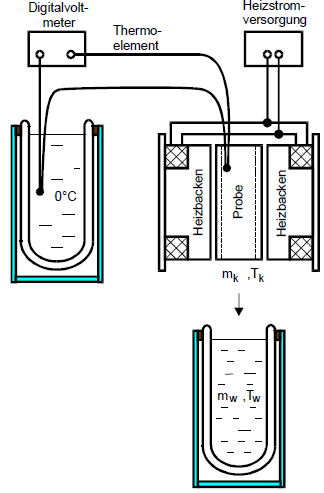
\includegraphics[scale=0.65]{Text/Bilder/Kalorimeter.png}
  \caption{Schematischer Aufbau des Kalorimeters \cite[158]{sample1}.}
  \label{fig:kalorimeter}
\end{figure}
Aufgrund des Temperaturunterschieds $\Delta T$ stellt sich eine Mischtemperatur $T_m$ ein.
Die vom Probenkörper abgegebene Wärmemenge $Q_1$ ist dann gegeben durch:
\begin{equation}
  Q_1=c_k m_k \cdot \left( T_k-T_m \right ).
\end{equation}
Für die vom Wasser und den Wänden des Kalorimeters aufgenommene Wärmemenge $Q_2$ gilt:
\begin{equation}
  Q_2=\left (c_w m_w + c_g m_g \right ) (T_m-T_w) ,
\end{equation}
wobei $c_w$ hier die spezifische Wärmekapazität des Wassers und $c_g m_g$ die Wärmekapazität des Kalorimeters ist.
Unter der Annahme, dass eine vernachlässigbare Wärmemenge an die Umgebung abgegeben oder aufgenommen wird
und das System keine Arbeit verrichtet, können die Wärmemengen gleichgesetzt werden und es ergibt sich der
Zusammenhang:
\begin{equation}
  c_k= \frac {c_w m_w + c_g m_g}{m_k} \cdot \frac{T_m-T_w}{T_k-T_m} \label{eqn:ck}
\end{equation}
Die Wärmekapazität des Kalorimeters kann mithilfe zweier Wassermengen der Massen $m_x$, $m_y$ und
Temperaturen $T_x$, $T_y$ bestimmt werden.
Unter den selben Vorraussetzungen, die bei \eqref{eqn:ck} anngenommen werden, lässt sich nun der Zusammenhang
\begin{equation}
  c_g m_g=\frac{c_w m_y \left(T_y-T'_m \right)-c_w m_x \left(T'_m-T_y \right)}{T'_m-T_y}
  \label{eqn:kal}
\end{equation}
herleiten. $T'_m$ ist dabei die Mischtemperatur der beiden Wassermengen.

\subsection{Das Dulong-Petitsche Gesetz}
Das Dulong-Petitsche Gesetz besagt, dass die aufgenommene Molwärme eines Körpers unabhängig von seinen
chemischen Eigenschaften immer $3R$ beträgt, wobei $R$ = \SI{8,31}{\joule\per\mol\per\kelvin} \cite{sample3} die allgemeine Gaskonstante ist.
Dies folgt aus der Annahme, dass Atome in Festkörpern harmonische Schwingungen durchführen, was zur Folge hat, dass
\begin{equation}
  \langle E_\text{kin} \rangle = \langle E_\text{pot} \rangle
\end{equation}
gilt.
Daraus folgt
\begin{equation}
  \langle U \rangle=\langle E_\text{kin} \rangle + \langle E_\text{pot} \rangle=2\langle E_\text{kin} \rangle
\end{equation}
Das Äquipartitionstheorem besagt, dass ein Atom im thermischen Gleichgewichtszustand bei absoluter
Temperatur $T$ pro Bewegungsfreiheitsgrad eine mittlere kinetische Energie von $\frac{1}{2} kT$ besitzt,
wobei $k$ die Boltzmannsche Konstante ist.
Daraus folgt:
\begin{equation}
  \langle U \rangle=kT
\end{equation}
Unter Berücksichtigung, dass ein Atom 3 Begwegungsfreiheitsgrade hat und dass sich in einem Mol $6,02\cdot 10^{23}$ Atome
befinden, folgt für die Molwärme
\begin{equation}
  C_V=3R
\end{equation}

\subsection{Quantenmechanische Methode}
Zwar strebt die Molwärme vieler Stoffe bereits bei Zimmertemperatur tatächlich gegen $3R$, jedoch fällt auf, dass
Stoffe mit geringen Atomgewicht erst bei hohen Temperaturen eine Molwärme von $3R$ erreichen.
Dieser Widerspruch zum Dulong-Petitschen Gesetz folgt aus der dort getroffenen Annahme, dass Atome bei
Schwingungen beliebige Energiebeträge aufnehmen oder abgeben können, was der Quantenmechanik widerspricht.
Laut dieser können mit $\omega$ oszillierende Atome nur gequantelte Energiemengen
\begin{align}
  \Delta U= n\cdot \hbar \cdot \omega
\end{align}
\begin{center}
 \small {(wobei n  $\in \mathbb{N}$ , $\hbar =\frac{h}{2\pi}$ und $h = \text{Planksches Wirkumsquantum}$)}
\end{center}
aufnehmen oder abgeben.
Daraus ergibt sich ein anderer Zusammenhang zwischen mittlerer Energie und Temperatur:
\begin{equation}
  \langle U_\text{qu} \rangle=\frac{3N \hbar \omega}{\exp{\frac{\hbar \omega}{kT}}-1}
\end{equation}
\begin{center}
 \small {(wobei $N=$ \SI {6,02 e23}{1\per\mol})}
\end{center}
Im Fall $kT \gg \hbar \omega$ strebt die Energie jedoch gegen $3R$.
Dies ist bei kleinen Massen aufgrund von $\omega \sim \frac{1}{\sqrt{m}}$ erst bei hohen Temperaturen der Fall.
